\chapter{Theoretische und technische Grundlagen}\label{ch:grundlagen}

Dieses Kapitel vermittelt die für das Verständnis der Arbeit erforderlichen Grundlagen. Es beginnt mit den zentralen Konzepten eingebetteter Systeme und der Bare-Metal-Programmier-ung.  Im Anschluss wird das deutsche Einhand-Fingeralphabet als zu erkennendes Zeichensystem eingeführt. Abschließend werden die Grundlagen des maschinellen Lernens, der \linebreak Handdetektion, der Modellquantisierung sowie der Edge AI erläutert.

\section{Eingebettete Systeme \& STM32N6570DK}\label{sec:eingebettete-systeme}
\subsection{Begriffsbildung und Merkmale}\label{sub:begriffsbildung-merkmale}

Eingebettete Systeme (engl. embedded systems) sind Computersysteme, die als Bestandteil eines übergeordneten Gesamtsystems in eine technische Umgebung eingebettet sind \cite[S. 2]{marwedel2021}. Im Gegensatz zu universellen Rechnern (Personal Computer, Server) erfüllen sie eine spezifische, fest definierte Aufgabe und sind darauf optimiert. Typische Merkmale sind:

\begin{table}[htbp]
    \centering
    \label{tab:embedded-merkmale}
    \begin{tabular}{|p{0.18\textwidth}|p{0.75\textwidth}|}
        \hline
        \textbf{Aspekt} & \textbf{Embedded-spezifisch} \\
        \hline
        Ressourcen-beschränkung & Eingebettete Systeme verfügen über begrenzten Arbeitsspeicher (RAM), begrenzten Programmspeicher (Flash) und eine eingeschränkte Rechenleistung im Vergleich zu General-Purpose-Computern. \\
        \hline
        Echtzeitfähigkeit & Viele Anwendungen erfordern, dass Daten innerhalb definierter Zeitgrenzen verarbeitet werden. Man unterscheidet zwischen \texttt{weicher} Echtzeit (eine Überschreitung der Frist ist unerwünscht, aber tolerierbar) und \texttt{harter} Echtzeit (eine Überschreitung führt zum Systemversagen). \\
        \hline
        Hohe \newline Zuverlässigkeit & Da eingebettete Systeme häufig in sicherheitskritischen oder industriellen Anwendungen eingesetzt werden, ist ein zuverlässiger und langfristig fehlerfreier Betrieb sicherzustellen. \\
        \hline
        Energieeffizienz & Viele Systeme arbeiten mit begrenzter Energieversorgung (Batterien, Netzteil), weshalb der Energieverbrauch eine zentrale Designrandbedingung darstellt. \\
        \hline
        Spezialisierung & Im Unterschied zu universellen Rechnern ist die Funktionalität eines eingebetteten Systems auf einen konkreten Anwendungsfall beschränkt. \\
        \hline
    \end{tabular}
    \caption{Charakteristische Merkmale eingebetteter Systeme \cite[S. ~3 ff.]{bernsteinMikrocontroller2026}}
\end{table}

\subsection{Mikrocontroller Architektur}\label{sub:mikrocontroller-architektur}

Als dominierende Hardwareplattform eingebetteter Systeme dienen Mikrocontroller (MCU, engl.\ \texttt{Microcontroller Unit}). Ein Mikrocontroller integriert auf einem einzigen Halbleiterchip alle für einen vollständigen Computer wesentlichen Komponenten \cite[S. ~3 ff.]{bernsteinMikrocontroller2026}:

\begin{itemize}
    \item CPU: Recheneinheit mit Instruktionssatz (z.\,B.\ Arm Cortex-M, RISC-V). Die Taktfrequenz bestimmt die Verarbeitungsgeschwindigkeit und reicht von wenigen MHz bis zu mehreren hundert MHz.
    \item Programmspeicher (Flash): Nichtflüchtiger Speicher für den Programmcode und konstante Daten. Die Größe variiert von einigen Kilobyte bis zu mehreren Megabyte.
    \item Arbeitsspeicher (RAM): Flüchtiger Speicher für Laufzeitdaten, Variablen und Stack. Typisch sind wenige Kilobyte bis einigen hundert Kilobyte.
    \item Taktgeber: Interner Oszillator \texttt{(HSI, engl.\ High-Speed Internal)} oder externer \linebreak Quarz \texttt{(HSE, engl.\ High-Speed External)} als Zeitbasis für die CPU und Peripherie.
    \item Peripherie-Einheiten: Hardwaremodule für Ein-/Ausgabe, Kommunikation und Zeit- \linebreak steuerung (siehe Abschnitt \ref{sub:peripherieschnittstellen}).
\end{itemize}

\begin{figure}[htbp]
    \centering
    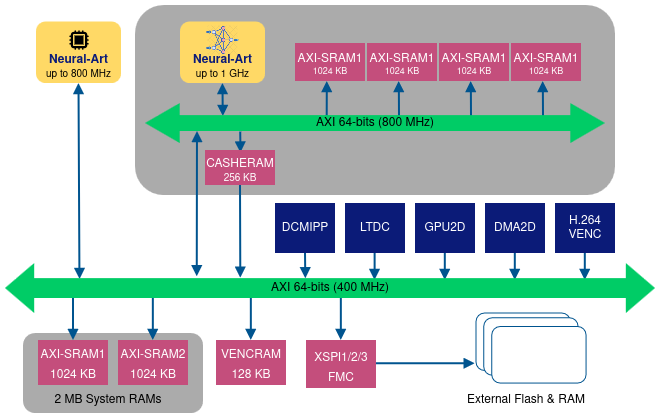
\includegraphics[width=0.9\textwidth]{material/figures/STM32N6-Architecture.drawio.png}
    \caption{STM32N6570-DK - Architektur | \cite{stmicroelectronics-learningSTM32N6DemoWorkshop2025}}
    \label{fig:stm32n6-architektur}
\end{figure}

\subsection{Peripherieschnittstellen}\label{sub:peripherieschnittstellen}

Mikrocontroller stellen verschiedene Hardware-Schnittstellen bereit, um mit der Umwelt zu interagieren. Die wesentlichen Peripherietypen sind \cite[S. ~48 ff, S. ~3104 ff., S. ~2153 ff., s. ~2093 ff]{bernsteinMikrocontroller2026, rm0486}:

\begin{itemize}
    \item General Purpose Input/Output (GPIO): GPIO-Pins sind die einfachste Form der digitalen Ein-/Ausgabe. Jeder Pin kann konfiguriert werden als Eingang (Lesen eines logischen Pegels: 0 oder 1) oder als Ausgang (Setzen eines Pegels). GPIO-Pins werden zum Ansteuern von LEDs, Auslesen von Tasten oder als Steuerleitungen für andere Peripheriemodule verwendet.
    \item  Universal Synchronous/Asynchronous Receiver/Transmitter (USART):  Serielles Kommunikationsprotokoll zur asynchronen Datenübertragung. Es wird für Debug-Ausgaben, die Kommunikation mit Host-PCs oder seriellen Sensoren eingesetzt.
    \item Serial Peripheral Interface (SPI): Synchrones, vollduplexes Kommunikationsprotokoll mit Transmitter-Receiver-Architektur. Es bietet höhere Datenraten als UART und wird bevorzugt für externe Speicher (Flash, PSRAM), Display-Controller oder Sensoren verwendet. Ein SPI-Bus besteht typischerweise aus den Leitungen COPI, CIPO, SCK und einem Chip-Select (CS).
    \item Inter-Integrated Circuit (I²C):  Zweidrahtiges, synchrones Kommunikationsprotokoll\linebreak (SDA, SCL) mit Adressierung. Es ermöglicht den Anschluss mehrerer Peripherals über denselben Bus und wird für Sensoren, Echtzeituhren (RTC) und kleinere EEPROMs verwendet.
    \item Timer: 
    Hardware-Timer zählen Taktimpulse und können Interrupts auslösen, wenn ein Zählerwert erreicht wird. Sie dienen als Zeitbasis für periodische Aufgaben, zur Erzeugung von PWM-Signalen (Pulsweitenmodulation) und zur Messung von Signalen (Input Capture). In Echtzeitsystemen stellen Timer den Taktgeber für den Scheduler dar.
    \item Direct Memory Access (DMA): DMA-Einheiten ermöglichen Datenübertragungen zwischen Peripherie und Speicher ohne CPU-Beteiligung. Die CPU gibt lediglich den Startbefehl und kann während der Übertragung andere Aufgaben verarbeiten. DMA ist besonders für große Datenströme (z.\,B.\ Kamerabilder) relevant, da es die CPU erheblich entlastet.
    \item DMA2D (ChromART):  Eine spezielle DMA-Einheit für 2D-Bild-Operationen: Kopieren, Füllen und Alpha-Blending von Bilddaten ohne die CPU zu blockieren (Erweiterung des DMA).
    \item Interrupts:  Interrupts ermöglichen es der CPU, auf asynchrone Ereignisse (z.\,B.\ Eingangsimpuls, abgeschlossene Datenübertragung, Timer-Überlauf) zeitnah zu reagieren, ohne den Ereigniszeitpunkt aktiv abfragen zu müssen. Der Interrupt-Controller (NVIC, engl.\ \texttt{Nested Vectored Interrupt Controller} bei Arm Cortex-M) verwaltet Prioritäten und erlaubt Verschachtelung (Nested Interrupts). Nach dem Speichern des laufenden Kontexts (Registersatz) springt die CPU über die Vektortabelle auf die zugehörige Interrupt-Service-Routine (ISR)\cite[S. 104 ff.]{yiuDefinitiveGuideARM2013}.
    \item External Interrupts (EXTI): Der EXTI-Controller erlaubt es, asynchrone Signale auf GPIO-Pins als Interrupts zu behandeln. Er eignet sich für Ereignisse wie Berührungen eines Touch-Controllers, Tastendrücke oder Flankenwechsel externer Sensoren und löst bei einem konfigurierten Ereignis die zugehörige ISR aus \cite[Kap. 7]{yiuDefinitiveGuideARM2013}.
    \item External Serial Peripheral Interface (XSPI): Hochgeschwindigkeits-Schnittstelle für den Anschluss externer Speicher wie PSRAM und NOR-Flash. Je nach Konfiguration werden vier (Quad-SPI) oder acht Datenleitungen (OctoSPI) verwendet. XSPI erlaubt neben dem seriellen Transfer auch die Einblendung der externen Speicher in den Adressraum des Prozessors (Memory-Mapped-Modus, siehe Abschnitt \ref{sub:speicherarchitektur}) \cite[S. 1288]{rm0486, STM32N6570DKProductSTMicroelectronics}.
    \item LCD-TFT Display Controller (LTDC): Controller zur Erzeugung des Bildsignals für ein LCD-Display. Er liest die Bilddaten kontinuierlich aus zugeordneten Speicherbereichen (Framebuffern) und kombiniert mehrere übereinanderliegende Layer mit unterschiedlichen Farbformaten und Alpha-Werten (Layer- und Alpha-Blending). Dadurch wird die CPU von der kontinuierlichen Displayaktualisierung entlastet \cite[S. 2093]{rm0486}.
    \item Camera Serial Interface (CSI): Serielle Schnittstelle zur Übertragung von Bilddaten eines Kamerasensors (z.\,B.\ MIPI-CSI). Sie überträgt die Rohdaten des Sensors (z.\,B.\ RAW-Bayer-Daten) zeilenweise an den Mikrocontroller \cite[S. 2015]{rm0486}.
    \item Digital Camera Interface Pixel Pipeline (DCMIPP): Hardware-Pipeline zur Verarbeitung des Kameradatenstroms. Sie übernimmt rechenintensive Bildverarbeitungsschritte wie Demosaikierung, Farbkorrektur, Gammakorrektur, Zuschnitt (Crop) und Skalierung (Downscale) und stellt das Ergebnis über mehrere parallele Ausgabepfade (Pipes) in unterschiedlichen Auflösungen und Formaten bereit \cite[S. 1815]{rm0486}.

\end{itemize}

\subsection{Speicherarchitektur}\label{sub:speicherarchitektur}

Die Speicherarchitektur eingebetteter Systeme weicht wesentlich von klassischen Rechnern ab. Die wesentlichen Speichertypen sind \cite{STM32N6570DKProductSTMicroelectronics, rm0486}:

\begin{itemize}
    \item Flash-Speicher (On-Chip): Nichtflüchtig, integriert auf dem MCU-Chip. Dient als Programmspeicher (Code) und für konstante Daten (Konstanten-Tabelle, lookup tables). Schreibzugriffe sind langsam und erfordern einen Löschzyklus.
    \item SRAM (On-Chip): Flüchtig, sehr schneller Zugriff (im Takt der CPU). Dient als Hauptspeicher für Variablen, Heap und Stack. Auf ausgewählten Cortex-Systemen ist SRAM in mehrere Banken aufgeteilt (AXISRAM), um parallele Zugriffe durch CPU, DMA und NPU zu ermöglichen.
    \item PSRAM (extern): Pseudo-Static RAM, angeschlossen über OctoSPI oder Quad-SPI. Bietet größere Speicherkapazitäten als On-Chip-SRAM bei moderater Zugriffszeit. Im STM32N6570-System wird PSRAM für Zwischenspeicherung von Bilddaten genutzt.
    \item NOR-Flash (extern): Nichtflüchtiger Speicher mit seitenweisem Zugriff, angeschlossen über OctoSPI.
\end{itemize}

Die Speicherhierarchie bestimmt maßgeblich die Systemleistung. Cortex-M55-Kerne verfügen über ein Cachesystem (I-Cache, D-Cache), das den Zugriff auf langsame externe Speicher beschleunigt. Da Peripherie-Einheiten (LTDC, DMA2D, GPU2D) jedoch häufig direkt auf den Speicher zugreifen, muss die Cache-Kohärenz manuell verwaltet werden (Flush/Invalidate) \cite[S. ~308ff.]{rm0486}.

Externe Speicher wie PSRAM und NOR-Flash werden über die XSPI-Schnittstellen angebunden und können im \textit{Memory-Mapped-Modus} direkt in den Adressraum des Mikrocontrollers eingeblendet werden. Lese- und Schreibzugriffe erfolgen dann über reguläre Speicheradressen, ohne dass für jede Transaktion separat eine Übertragung über die Schnittstelle angestoßen werden muss. \cite[S. 1288]{rm0486}.

Bilddaten für Display oder Bildverarbeitung werden üblicherweise in zusammenhängenden Speicherbereichen, den \textit{Framebuffern}, gehalten. Um zu verhindern, dass ein Bild überschrieben wird, während es noch angezeigt oder verarbeitet wird, kommen mehrere Puffer zum Einsatz. Beim \textit{Double-Buffering} werden zwei Puffer abwechselnd befüllt und ausgegeben: Während ein Puffer mit neuen Daten beschrieben wird, kann der andere bereits für die Ausgabe genutzt werden.

\subsection{Clock-Systeme}\label{sub:clock-systeme}

Das Clock-System bestimmt die Taktfrequenz aller Komponenten und ist eine fundamentale Voraussetzung für den Betrieb des Mikrocontrollers \cite[S. ~411 ff.]{STM32N6570DKProductSTMicroelectronics, rm0486}.

\begin{itemize}
    \item Oszillatoren: Der interne Hochgeschwindigkeitsoszillator (HSI) bietet eine integrierte, quarzfreie Takquelle (typisch 16--64\,MHz). Externe Quarze (HSE) liefern eine höhere Genauigkeit und Stabilität.
    \item PLL (Phase-Locked Loop): Ein PLL multipliziert die Taktfrequenz der Basisoszillatoren auf höhere Taktfrequenzen. Das STM32N6570-System verwendet mehrere PLLs: PLL1 für den CPU-Takt (800\,MHz), PLL2 für den NPU (1000\,MHz), PLL3 für den NPU-Speicher (900\,MHz) und PLL4 für Peripherietakte.
    \item Takthierarchie: Der PLL-Ausgang wird über Teiler (Prescaler) auf verschiedene Busdomänen verteilt: AHB (High-Speed Bus), APB1/APB2 (Peripheral Buses). Peripherie-Einheiten erhalten ihren Takt von diesen Bussen.
\end{itemize}

\subsection{Bare-Metal-Programmierung}\label{sub:bare-metal}

\paragraph{Definition und Abgrenzung:}
Als Bare-Metal-Programmierung bezeichnet man die Softwareentwicklung auf einem Mikrocontroller ohne Einsatz eines Betriebssystems (OS) oder Echtzeitbetriebssystems (RTOS) \cite[Kap. ~2]{GbatiIsrael2024BECP}. Der Programmcode hat direkten Zugriff auf die Hardwareregister, und die Ausführungsreihenfolge wird vollständig durch den eigenen Code bestimmt. Dies steht im Gegensatz zu OS-basierter Programmierung, bei der ein Betriebssystem (z.\,B.\ FreeRTOS, Zephyr) die Ressourcenverwaltung, Scheduling und Synchronisierung übernimmt.

\paragraph{Startup und Systeminitialisierung:}
Nach dem Einschalten oder Reset beginnt die CPU an einer durch die Vektor-Tabelle definierten Adresse (Reset-Handler). Der Startup-Code führt folgende Schritte aus: (1) Kopieren der Initialisierungsdaten aus Flash nach SRAM (.data-Sektion), (2) Löschen der .bss-Sektion (uninitialisierte globale Variablen), (3) Konfiguration des Stack-Pointers, (4) Aufruf der main-Funktion. Die Vektor-Tabelle enthält außerdem Adressen aller Interrupt-Handler (Exceptions).

\paragraph{Linker-Skript und Boot-Prozess:}
Die Zuordnung von Code und Daten zu den Speicherregionen erfolgt über das Linker-Skript. Es legt die verfügbaren Speicherbereiche (ROM, RAM, externe Speicher), deren Basisadressen und Größen sowie die Platzierung der einzelnen Sektionen fest \cite[Kap. ~2.4]{yiuDefinitiveGuideARM2013}. Da der STM32N657x0 über keinen internen Flash verfügt, wird die Firmware als First-Stage-Bootloader-Binary (FSBL) in das On-Chip-SRAM geladen und von dort ausgeführt. \cite[S. ~286 ff., S. ~183 ff.]{rm0486}

\paragraph{Register-Level-Programmierung:}
Bei der Register-Level-Programmierung werden Peripherieeinheiten durch direkten Zugriff auf die Memory-Mapped-I/O-Register (MMIO) des Mikrocontrollers konfiguriert. Jedes Register hat eine fest definierte Adresse im Speicherbereich. Die Konfiguration erfolgt durch Setzen oder Löschen einzelner Bits mit Bitmasken. Beispielsweise wird ein GPIO-Pin als Ausgang konfiguriert, indem im Mode-Register die entsprechenden Bits gesetzt werden. Der Vorteil gegenüber einer Hardware-Abstraktionsschicht (HAL) liegt in der vollen Kontrolle über die Ausführungszeit und den Speicherverbrauch. \cite[Kap. ~2]{GbatiIsrael2024BECP}

\paragraph{CMSIS:}
Der Cortex Microcontroller Software Interface Standard (CMSIS) ist eine von Arm bereitgestellte Sammlung standardisierter Prozessor- und Gerätedefinitionen für Cortex-Mikro\-controller \cite{CMSISIntroduction}. Sie umfasst unter anderem die Registerstrukturen der Peripherie, die Definition der Interruptnummern sowie Funktionen für den Zugriff auf den Prozessorkern. Die registerbasierte Programmierung des vorliegenden Projekts stützt sich auf diese Definitionen. \cite[Kap. ~2.9]{yiuDefinitiveGuideARM2013}

\paragraph{Resource Isolation Framework Security Controller (RIFSC):}
Der RIFSC verwaltet die Zugriffsrechte und Sicherheitsattribute auf interne Speicherbereiche und Peripheriekomponenten des STM32N6570. Eine fehlerhafte Konfiguration kann verhindern, dass Komponenten trotz aktiver Taktversorgung auf die benötigten Register zugreifen können. Die Zugriffsrechte werden daher eingerichtet, bevor die jeweiligen Hardwarekomponenten initialisiert werden \cite{ResourceIsolationFramework}.

\paragraph{Software-Scheduling:}
Eingebettete Software ohne Betriebssystem muss die Ausführung mehrerer Aufgaben selbst organisieren. Der einfachste Ansatz ist die \textit{Super-Loop}, eine sequenzielle Schleife, die alle Aufgaben nacheinander abarbeitet. Dies genügt nur, wenn alle Aufgaben innerhalb ihrer Zeitgrenzen ausgeführt werden können \cite[Kap. 2.5]{yiuDefinitiveGuideARM2013}. Andernfalls kommen Scheduler zum Einsatz:
\begin{itemize}
    \item Scheduler-Arten: Der \textit{Round-Robin-Scheduler} vergibt die CPU zyklisch an bereite Aufgaben (Tasks). Ein \textit{prioritätsbasierter präemptiver Scheduler} unterbricht (preemptiert) laufende Aufgaben zugunsten höherpriorisierter Tasks.
    \item Task-Zustände: Ein Task durchläuft typischerweise mehrere Zustände, etwa \textit{Ready} (bereit zur Ausführung), \textit{Blocked} (wartend) und \textit{Suspended} (angehalten).
    \item Kontextwechsel: Der Wechsel zwischen Aufgaben wird als Context Switch bezeichnet. Der Zustand der unterbrochenen Aufgabe (Register, Stack) wird gesichert und der Zustand der nächsten Aufgabe wiederhergestellt. Auf Arm-Cortex-M-Prozessoren erfolgt der initiale Start über einen Supervisor Call (SVC), der eigentliche Wechsel über den PendSV-Interrupt. Der Prozessor unterscheidet zwischen dem Main Stack Pointer (MSP) für Interruptkontexte und dem Process Stack Pointer (PSP) für Aufgabenkontexte. Über das Process Stack Limit Register (PSPLIM) wird die Stack-Grenze überwacht. Bei Nutzung der FPU werden die Gleitkommaregister nur dann gesichert, wenn sie tatsächlich verwendet wurden (Lazy Stacking) \cite[S. 28 ff.]{valvanoRealtimeOperatingSystems2017}.
    \item WFI: Im Leerlauf kann die CPU mit der Instruktion \texttt{WFI} (Wait For Interrupt) in einen energiearmen Wartezustand versetzt werden, aus dem sie erst durch ein Interrupt-Ereignis aufgeweckt wird. \cite[S. ~369]{rm0486}
    \item Fault-Handling: Aufgetretene Ausnahmezustände werden in mehrere Fault-Klassen unterteilt: \textit{HardFault} als zentraler Abfang-Interrupt sowie \textit{UsageFault}, \textit{BusFault} und \textit{MemManage Fault} für spezifische Fehlerursachen (ungültige Befehle, Speicherzugriffsfehler, MPU-Verletzungen). \cite[Kap. ~12]{yiuDefinitiveGuideARM2013}
    \item Zyklenmessung: Der DWT (Data Watchpoint and Trace) des Cortex-M55 stellt mit dem Zähler \texttt{CYCCNT} eine zyklen-genaue Zeitmessung bereit, mit der die Ausführungszeiten einzelner Tasks gemessen werden können. \cite[S. ~4422]{rm0486}
\end{itemize}

\paragraph{Vorteile und Trade-Offs:}
Bare-Metal ermöglicht minimale Latenz, minimalen Speicherverbrauch und deterministisches Verhalten. Die Nachteile liegen in der höheren Entwicklungskomplexität: Es gibt kein Thread-Management, keine Synchronisationsprimitive und keine automatische Ressourcenverwaltung. Für ressourcenbeschränkte Systeme mit linear definiertem Ablauf überwiegen jedoch die Vorteile.

\subsection{Hardware-Beschleunigung}\label{sub:hardware-beschleunigung}

Neben der CPU stehen dedizierte Hardware-Einheiten zur Verfügung, die bestimmte Operationen mit hoher Effizienz ausführen:

\begin{itemize}
    \item DMA: Entlastet die CPU bei Datenübertragungen.
    \item DMA2D: Übernimmt 2D-Bildoperationen (Kopieren, Skalieren, Füllen) ohne CPU-Beteil-igung.
    \item NPU (Neural Processing Unit): Dedizierter Beschleuniger für neuronale Netze. Die NPU führt Matrix-Multiplikationen und Aktivierungsfunktionen mit hoher Parallelität aus und erreicht dabei deutlich höhere Energieeffizienz als die allgemeine CPU. Im STM32 N6570\-DK arbeitet die NPU mit einer Taktfrequenz von bis zu 1000\,MHz und nativer INT8-Arithmetik \cite[S. 1011 ff.]{rm0486}.
\end{itemize}

\section{Deutsches Einhand-Fingeralphabet}\label{sec:fingeralphabet}

\subsection{Gebärdensprache als eigenständige Sprache}\label{sub:gebaerdensprache}
Gebärdensprachen sind natürlich entstandene, vollwertige Sprachen, die auf visuell-manuell-en Mitteln basieren. Sie unterscheiden sich von Lautsprachen nicht nur in der Modalität (Gestik und Mimik statt Laut und Klang), sondern verfügen über eigene grammatische Strukturen, Syntax und Semantik. Gebärdensprachen sind eigenständige Sprachen und keine abgeleiteten oder vereinfachten Formen der jeweiligen Lautsprache. \cite{DeutscheGebaerdensprache}

Die deutsche Gebärdensprache (DGS) ist die natürlich entstandene Sprache der Gehörlosengemeinschaft in Deutschland. Sie wird vor allem von gehörlosen und schwerhörigen Menschen sowie von deren Angehörigen und Gebärdensprachdolmetschern verwendet. Die DGS unterscheidet sich wesentlich von der deutschen Lautsprache in Grammatik, Satzbau und Ausdruck. Gebärdensprachliche Äußerungen bestehen aus einer Kombination von Handformen, Handbewegungen, Handpositionen im Raum sowie Mimik und Körpersprache. \cite{DeutscheGebaerdensprache}

\subsection{Das Fingeralphabet}\label{sub:fingeralphabet-detail}
Das Fingeralphabet ist ein Teilgebiet der deutschen Gebärdensprache \cite{aktion-mensch, DeutscheGebaerdensprache}. Es dient dem Buchstabieren einzelner Wörter und wird verwendet, wenn für ein Wort keine eigene Gebärde existiert. Etwa bei Eigennamen, Fachbegriffen oder bei der Kommunikation mit hörenden Gesprächspartnern. Im Gegensatz zur vollständigen Gebärdensprache beschränkt sich das Fingeralphabet auf die Darstellung von Handformen ohne Begleitung durch Mimik oder Bewegung im Raum. \cite{DeutscheGebaerdensprache}

\subsection{Das deutsche Einhand-Fingeralphabet}\label{sub:deutsches-fingeralphabet}
Das Fingeralphabet Umfasst die folgenden 29 Buchstaben: \texttt{A, B, C, D, E, F, G, H, I, J, K, L, M, N, O, P, Q, R, S, T, U, V, W, X, Y, Z, Ä, Ö, Ü}.  Zudem existiert ein Sonderzeichen \texttt{SCH} (als Trigraph dargestellt, d.h. ein Zeichen für drei Buchstaben) \cite{aktion-mensch}

\begin{figure}[H]
    \centering
    
\includegraphics[width=0.5\textwidth]{material/figures/aktion-mensch-deutsches-fingeralphabet.jpg}
    \caption{Deutsches Einhand-Fingeralphabet \cite{aktion-mensch}}
    \label{fig:fingeralphabet}
\end{figure}


\subsection{Handpositionen und Fingerkonfigurationen}\label{sub:handpositionen}

Jedes Zeichen des Fingeralphabets wird durch eine spezifische Konfiguration der Hand charakterisiert, die sich aus mehreren Parametern zusammensetzt \cite{aktion-mensch}:

\begin{itemize}
    \item Beteiligte Finger: Welche Finger sind gestreckt, welche sind gebeugt oder angeballt?
    \item Fingerkonfiguration: Sind Finger zusammengedrückt oder gespreizt?
    \item Daumenposition: Liegt der Daumen über den Fingern, neben ihnen, oder ist er abgespreizt?
    \item Handfläche: Zeigt die Handfläche zum Betrachter (ventral) oder weg (dorsal)?
    \item Fingerstellung: Zeigen die Finger nach oben, unten oder zur Seite?
\end{itemize}

Beispielhafte Beschreibung einiger Zeichen:

\begin{longtable}{|c|p{0.85\textwidth}|}
    \hline
    \textbf{Zeichen} & \textbf{Handkonfiguration} \\
    \hline
    \endfirsthead

    \hline
    \textbf{Zeichen} & \textbf{Handkonfiguration} \\
    \hline
    \endhead

    \hline
    \multicolumn{2}{r}{\textit{Fortsetzung auf nächster Seite}} \\
    \endfoot
    \caption{Personenspezifische Zuweisung der Kapitel}
    \label{tab:kapitelzuweisung}
    \endlastfoot

    A & Faust geschlossen, Daumen liegt seitlich an der Handfläche an. \\
    \hline
    B & Vier Finger gestreckt und zusammen, Daumen auf die Handfläche geklappt. \\
    \hline
    C & Alle Finger gebeugt, Hand formt eine C-förmige Öffnung. \\
    \hline
    E & Alle Finger auf den Daumen geklappt, Daumen sichtbar unter den Fingerspitzen. \\
    \hline
    I & Nur kleiner Finger gestreckt, übrige Finger geballt. \\
    \hline
    L & Daumen und Zeigefinger im 90°-Winkel gestreckt, übrige Finger geballt. \\
    \hline
    S & Faust geschlossen, Daumen vor den Fingern gekreuzt. \\
    \hline
    Y & Daumen und kleiner Finger gestreckt, übrige Finger geballt. \\
    \hline
    SCH & Alle Finger vom Handballen weggestreckt. \\
    \hline
\end{longtable}

\section{Grundlagen des maschinellen Lernens}\label{sec:ml-grundlagen}
\subsection{Begriffsbildung}\label{sub:ml-begriffsbildung}

Maschinelles Lernen \textit{(ML, engl. machine learning)} ist ein Teilgebiet der künstlichen Intelligenz, das Systeme befähigt, in Daten komplexe Muster und Zusammenhänge zu lernen und darauf basierend Vorhersagen oder Entscheidungen zu treffen, ohne explizit programmiert zu werden Anstelle fester Regeln wird dem Algorithmus ein Trainingsdatensatz zur Verfügung gestellt, aus dem er statistische Muster und Zusammenhänge ableitet. \cite[Kap. ~1.4]{MachineLearning1st}

\subsection{Supervised Learning}\label{sub:supervised-learning}

Beim überwachten Lernen  \textit{(supervised learning)} wird dem Modell ein Datensatz bestehend aus Eingabedaten \textit{(Features/Feature-Vektor)} und zugehörigen korrekten Ausgaben \textit{(Labels)} präsentiert \cite[S. ~9, Kap. ~1.5]{hastieElementsStatisticalLearning2009, MachineLearning1st}. Das Modell lernt, eine Funktion $f: X \rightarrow Y$ zu approximieren, die Eingaben auf die zugehörigen Ausgaben abbildet.

\subsection{Klassifikation}\label{sub:klassifikation}

Klassifikation ist ein zentrales Teilgebiet des maschinellen Lernens, bei dem die Aufgabe besteht, eine Eingabe einer von diskreten Klassenzugehörigkeiten zuzuordnen. Das Modell produziert für jede Klasse einen Wahrscheinlichkeitswert, und die Klasse mit der höchsten Wahrscheinlichkeit wird als Vorhersage ausgegeben. Typischerweise werden die Klassen innerhalb des Datensatzes mit Hilfe des One-Hot-Formats dargestellt \cite[Kap. ~2.7]{hastieElementsStatisticalLearning2009}.

\subsubsection{One-Hot-Format}\label{ssub:one-hot-format}

Beim One-Hot-Format werden Klassen durch Binärvektoren dargestellt, deren Länge der Anzahl aller möglichen Klassen entspricht. Dabei wird genau ein Eintrag des Vektors auf den Wert 1 gesetzt, welcher die zugehörige Klasse repräsentiert, während alle übrigen Einträge den Wert 0 annehmen. Beispielsweise wird bei drei möglichen Klassen die zweite Klasse durch den Vektor $[0,,1,,0]$ dargestellt. Diese Repräsentation ermöglicht eine eindeutige numerische Darstellung diskreter Klassen.
\cite{OneHotEncoder}

\subsubsection{Sparse Categorical Crossentropy}\label{ssub:sparse-cce}

Das One-Hot-Format verbraucht bei Hunderten von Klassen viel Speicherplatz. Sparse categorical Crossentropy löst dieses Problem indem der Datensatz einen einzigen Integer-Wert annimmt und die mathematisch äquivalente Kreuzentropie-Berechnung Speichereffizient im Hintergrund durchführt. \cite{SparseCategoricalCrossentropy18:23:14+00:00, WhatSparseCategorical10:49:00+00:00}

\begin{table}[H]
    \centering
    \label{tab:one-hot-codierung}
    \begin{tabular}{|l|c|c|}
        \hline
        \textbf{Kategorie} & \textbf{Index} & \textbf{One-Hot-Vektor} \\
        \hline
        NONE & 0 & [1, 0, 0, 0, 0] \\
        \hline
        A & 1 & [0, 1, 0, 0, 0] \\
        \hline
        B & 2 & [0, 0, 1, 0, 0] \\
        \hline
        C & 3 & [0, 0, 0, 1, 0] \\
        \hline
        D & 4 & [0, 0, 0, 0, 1] \\
        \hline
    \end{tabular}
    \caption{One-Hot-Kodierung vs.\ Sparse Indexdarstellung}
\end{table}

\subsection{Alternative Klassifikationsverfahren}\label{sub:alternative-klassifikatoren}

Neben neuronalen Netzen existieren weitere etablierte Klassifikationsverfahren, die im Rahmen der Modellauswahl in Betracht gezogen wurden:

\begin{itemize}
    \item Random Forest: Random Forests sind Ensemblemethoden, die eine Vielzahl von Entscheidungsbäumen kombinieren. Jeder Baum wird auf einer zufälligen Teilmenge der Trainingsdaten und Merkmale trainiert. Die Klassifikation erfolgt durch Mehrheitsabstimmung über alle Bäume. Random Forests sind robust gegenüber Overfitting und erfordern keine aufwendige Merkmalskalierung, geben jedoch nur harte Klassenzuordnungen und keine nativ kalibrierten Wahrscheinlichkeiten aus \cite[S. ~1 ff.]{rahmanComparisonSVMRandom2025}.
    \item Support Vector Machines (SVM): SVMs trennen Klassen durch eine Hyperebene im Merkmalsraum, die den Abstand zu den nächstliegenden Trainingspunkten (Support Vectors) maximiert. Über den Kernel-Trick lassen sich auch nichtlinear trennbare Daten verarbeiten. SVMs liefern ohne zusätzliche Kalibrierung keine Wahrscheinlichkeiten. Zur Umrechnung der Diskriminanzwerte in Wahrscheinlichkeiten ist ein nachgelagertes Platt-Scaling erforderlich \cite[S. ~1 ff.]{rahmanComparisonSVMRandom2025}.
\end{itemize}

\subsection{Metriken}\label{sub:metriken}

Zur Bewertung eines Klassifikationsmodells werden verschiedene Metriken herangezogen \cite[S. ~54 ff.]{fritzHandGestureRecognition}:

\begin{itemize}
    \item Accuracy (Genauigkeit): Anteil der korrekten Vorhersagen an allen Vorhersagen. Für ausgewogene Datensätze aussagekräftig, bei unausgewogenen Klassen jedoch irreführend.
    \item Konfusionsmatrix: Tabelle, die die tatsächlichen Klassen den vorhergesagten Klassen gegenüberstellt. Sie macht sichtbar, welche Zeichen miteinander verwechselt werden.
\end{itemize}

\begin{table}[H]
    \centering
    \label{tab:confusion-matrix-definition}
    \begin{tabular}{|l|l|l|}
        \hline
        & \textbf{Predicted 0} & \textbf{Predicted 1} \\
        \hline
        \textbf{Actual 0} & True Negative & False Positive \\
        \hline
        \textbf{Actual 1} & False Negative & True Positive \\
        \hline
    \end{tabular}
    \caption{Konfusionsmatrix -- Begriffsdefinitionen}
\end{table}


\subsection{Overfitting und Gegenmaßnahmen}\label{sub:overfitting}

Overfitting liegt vor, wenn ein Modell die Trainingsdaten zu gut lernt und dabei spezifische Muster, Rauschen und Ausreißer mitinterpretiert, diese allerdings nicht für die Allgemeingültigkeit relevant sind. Das Modell performt auf Trainingsdaten exzellent (Hohe Genauigkeit), auf unbekannten Daten jedoch schlecht (Geringe Genauigkeit).
\cite{yingOverviewOverfittingIts2019}

Gegenmaßnahmen bezüglich Overfitting umfassen:

\begin{itemize}
    \item Regularisierung: Bestrafung großer Gewichtswerte, um die Modellkomplexität zu begrenzen.
    \item Dropout: Zufälliges Deaktivieren eines Teils der Neuronen während des Trainings, um Abhängigkeiten zwischen Neuronen zu reduzieren.
    \item Datenaugmentation: Künstliche Vermehrung der Trainingsdaten durch Transformationen (siehe Abschnitt \ref{sec:augmentation-quantisierung}).
    \item Validierung: Aufteilen des Datensatzes in Trainings-, Validierungs- und Testset, um die Generalisierungsfähigkeit zu überwachen.
\end{itemize}

\subsection{Parameter vs Hyperparameter}\label{sub:parameter-hyperparameter}

Parameter sind Variablen welche aus dem zur Verfügung gestellten Datensatz beim Training erlernt werden. Diese werden nicht durch den Programmierer festgelegt. Hyperparameter hingegen werden vor dem Trainingsprozessen bestimmt. Diese Parameter bestimmen das Lernverhalten \cite[Kap. ~2.6]{burkovMachineLearningKompakt2019}.

\section{Neuronale Netze zur Klassifikation}\label{sec:neuronale-netze}
\subsection{Künstliche Neuronale Netze}\label{sub:knn}

Ein künstliches neuronales Netz (KNN) ist ein mathematisches Modell, das lose von biologischen neuronalen Netzen inspiriert ist \cite[S. ~1 ff.]{gurneyIntroductionNeuralNetworks2018}. Es besteht aus einer Menge von künstlichen Neuronen (auch Einheiten oder Knoten genannt), die in Schichten organisiert sind. Jedes Neuron berechnet eine gewichtete Summe seiner Eingaben, addiert einen Bias-Wert und wendet eine Aktivierungsfunktion an:

\begin{figure}[!h]
    \centering
    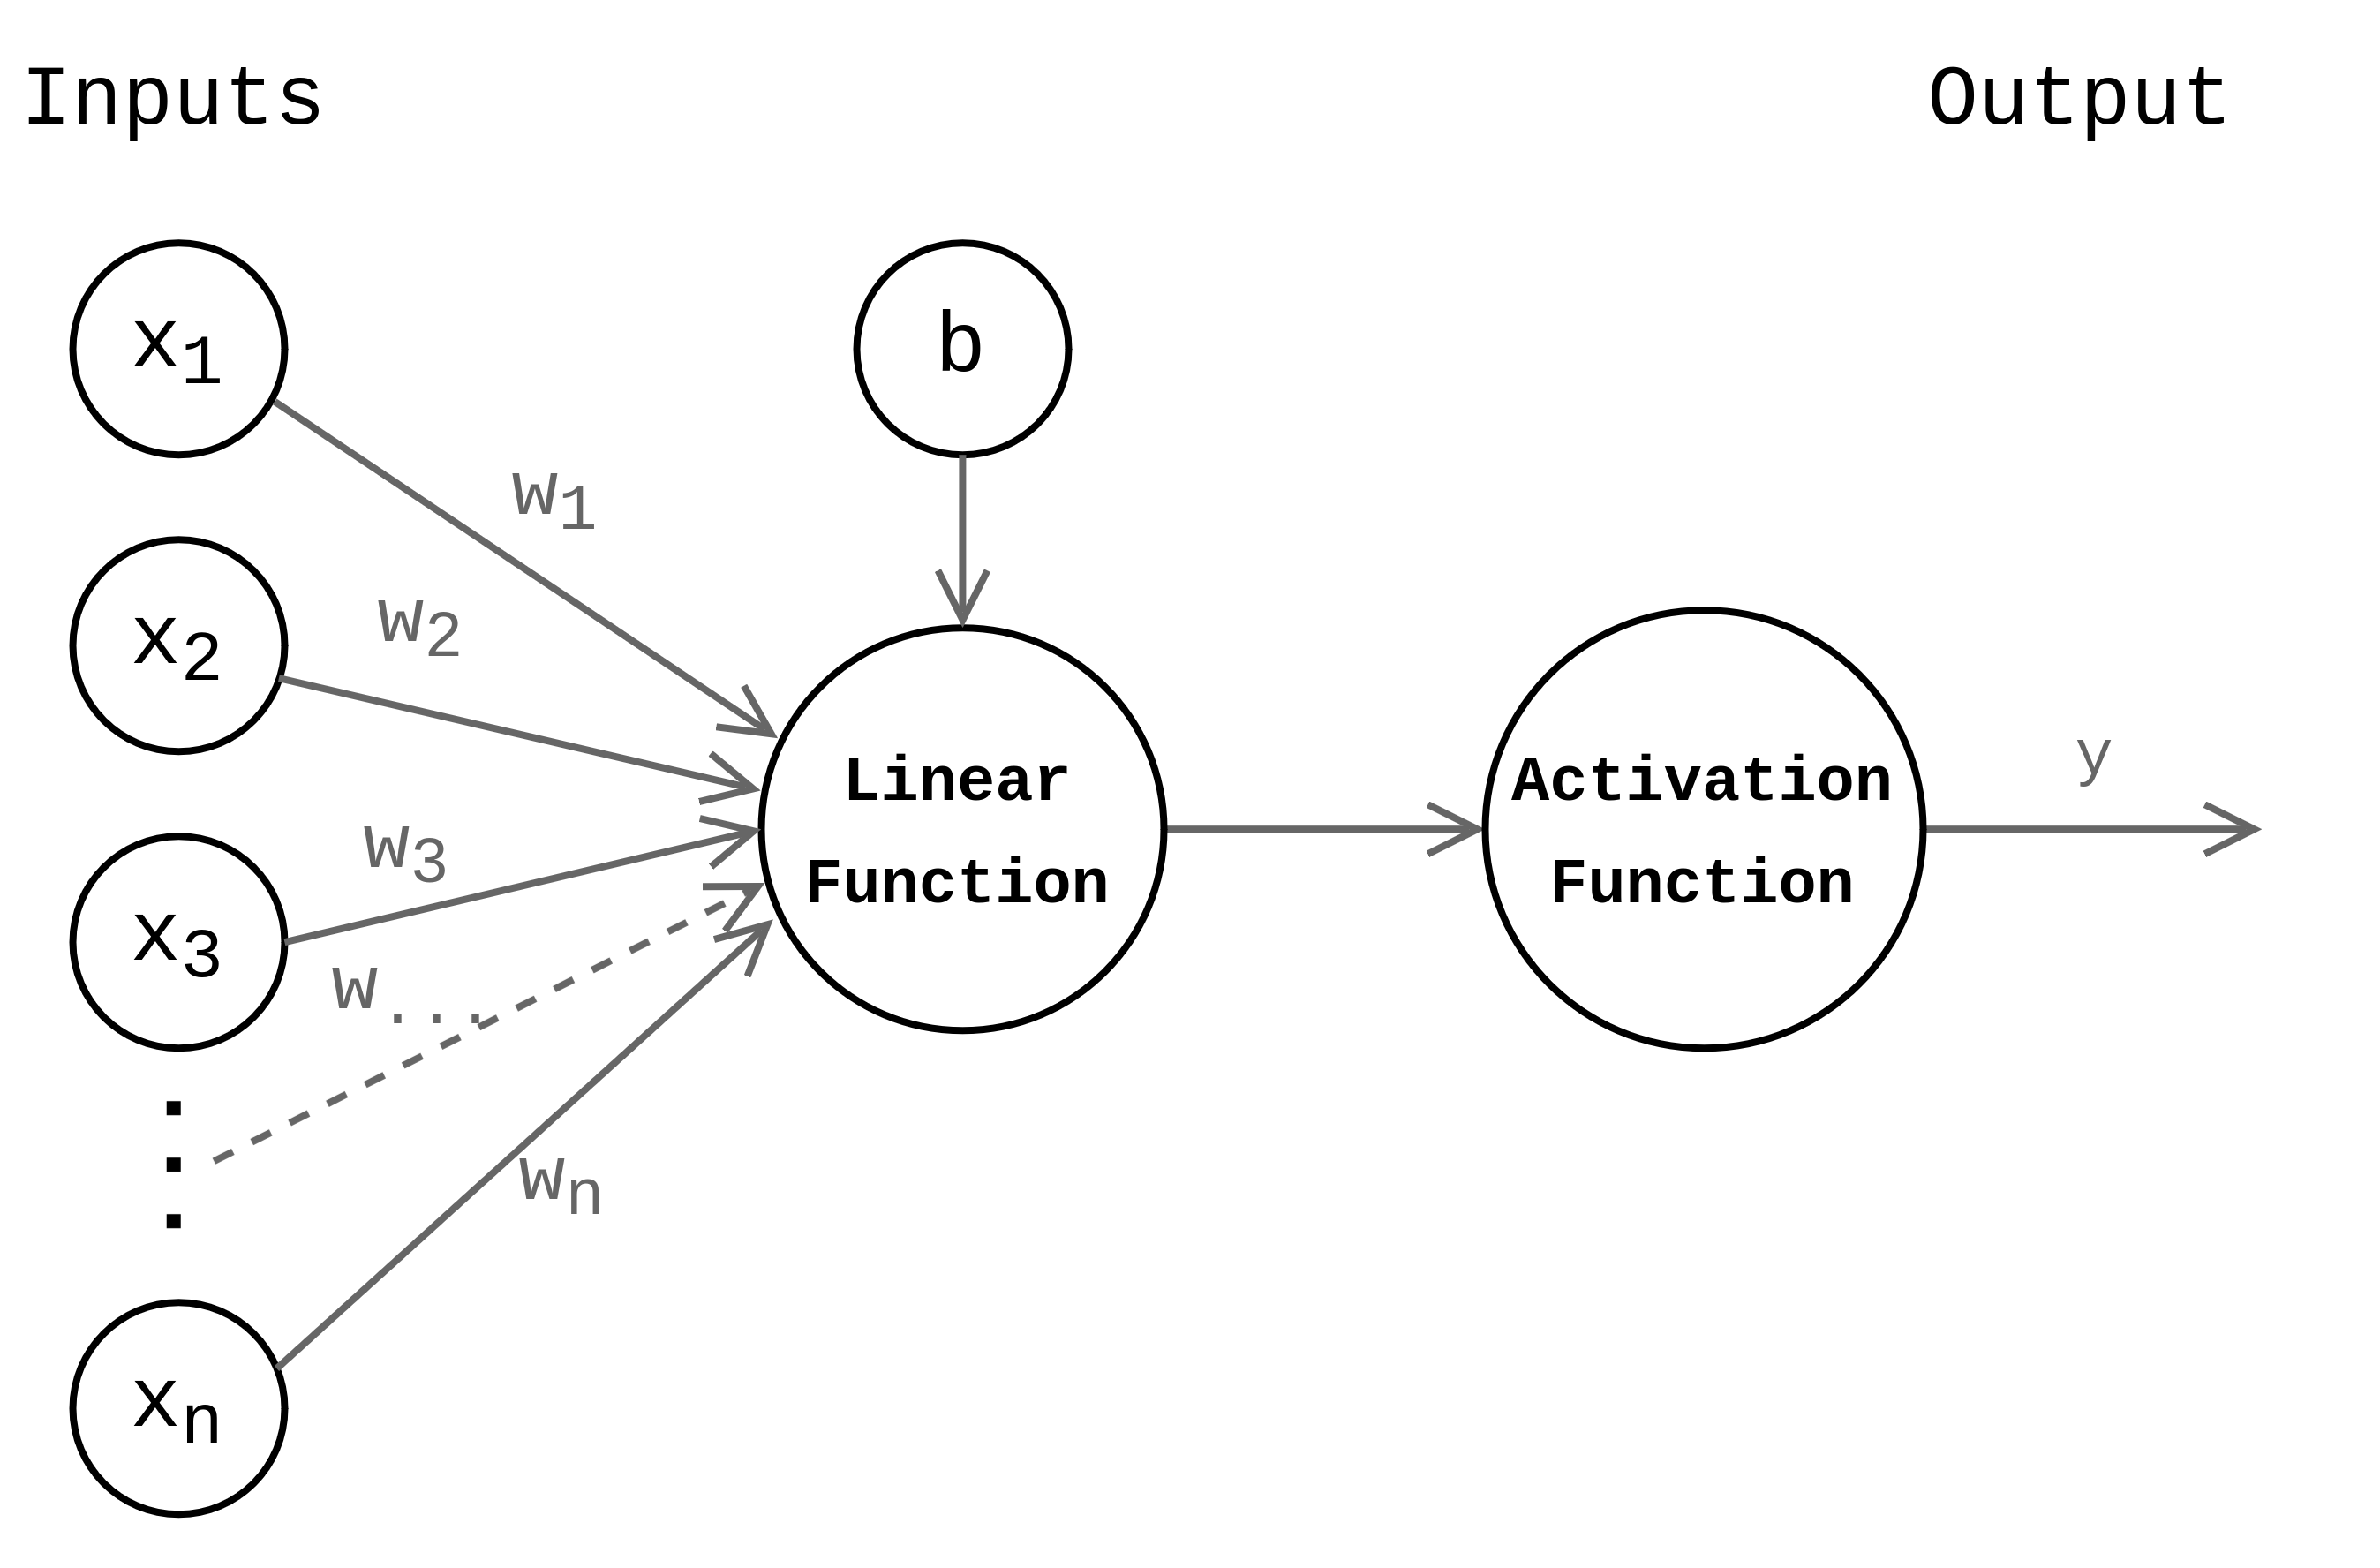
\includegraphics[width=0.9\textwidth]{material/figures/Neuron.drawio.png}
    \caption{Mathematisch modelliertes Neuron \cite[S. ~2]{gurneyIntroductionNeuralNetworks2018} | Eigene Darstellung}
    \label{fig:neuron}
\end{figure}

$$y = f\left(\sum_{i=1}^{n} w_i \cdot x_i + b\right)$$

wobei $x_i$ die Eingaben, $w_i$ die Gewichte, $b$ der Bias und $f$ die Aktivierungsfunktion sind.

\begin{figure}[!h]
    \centering
    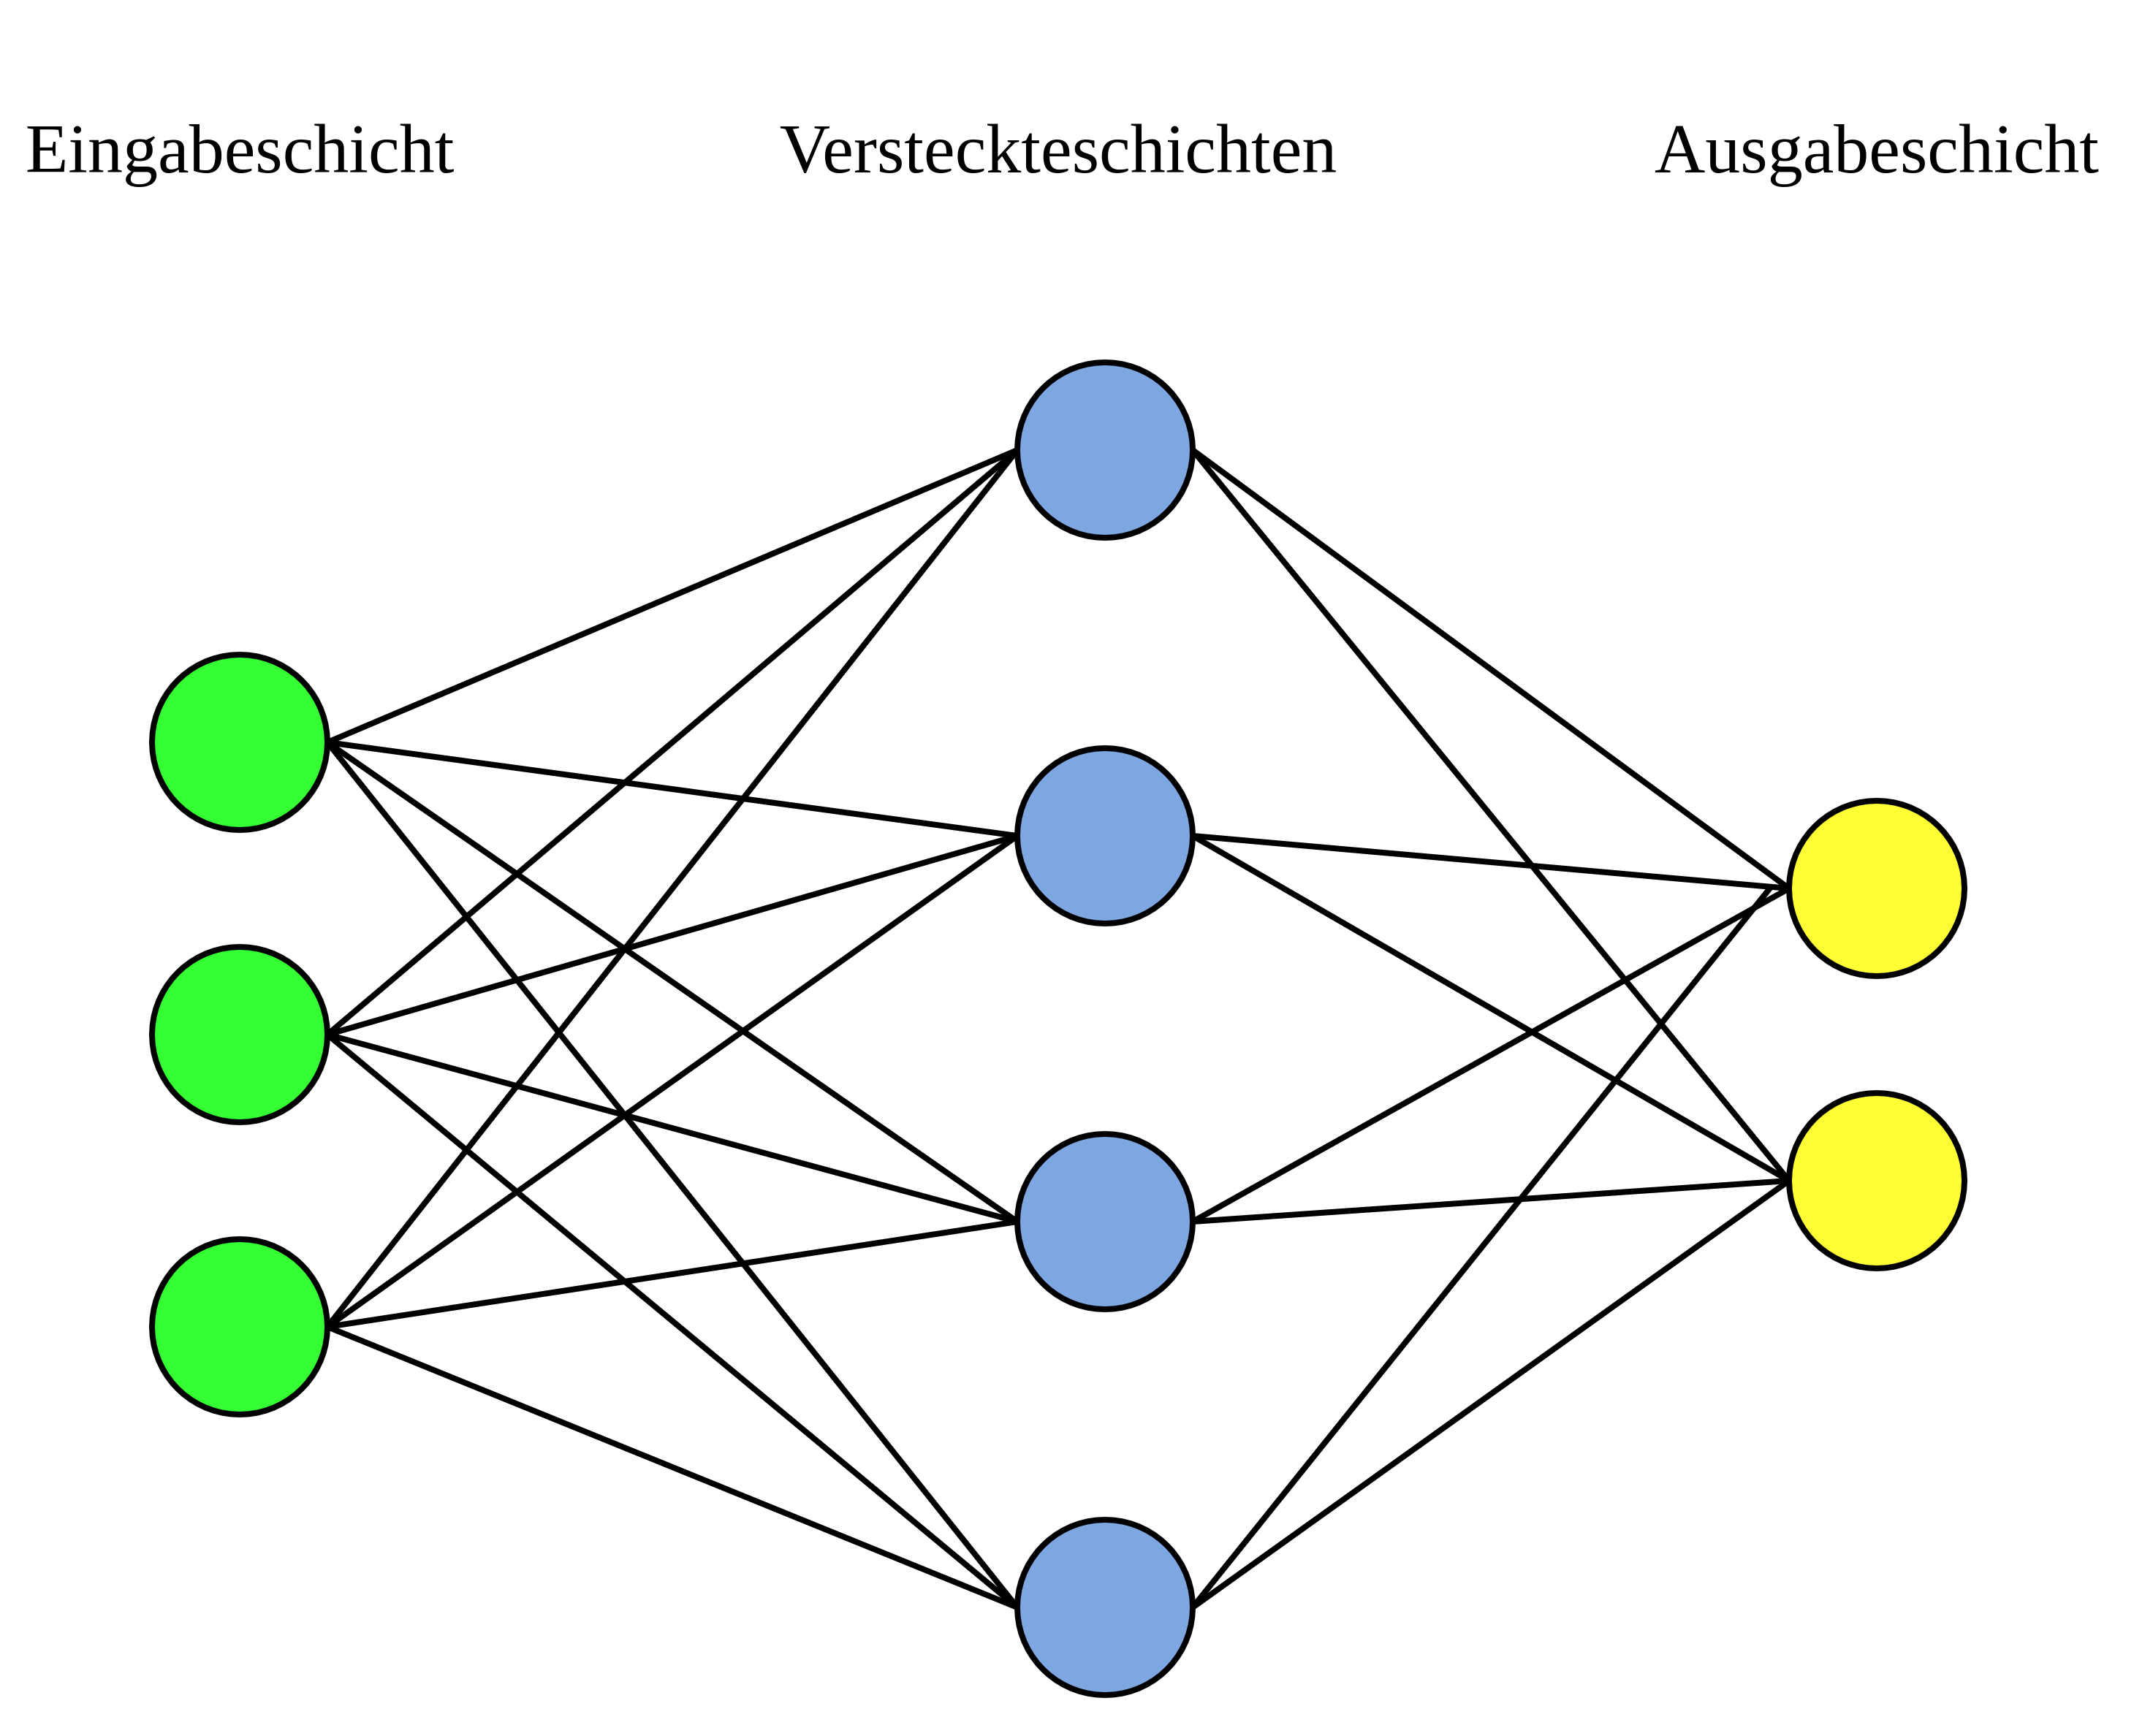
\includegraphics[width=0.9\textwidth]{material/figures/ML-Schichten.drawio.png}
    \caption{Allgemeine Struktur Künstlicher Neuronaler Netze | Eigene Darstellung}
    \label{fig:ml-schichten}
\end{figure}

\subsection{Aktivierungsfunktionen}\label{sub:aktivierungsfunktionen}

Aktivierungsfunktionen fügen Nichtlinearität in das Netz ein und ermöglichen es, komplexe Muster zu erlernen. Die wesentlichen im Projekt verwendeten Funktionen sind \cite[S. 310 ff.]{sharmaACTIVATIONFUNCTIONSNEURAL2020}:

\begin{itemize}
    \item ReLU (Rectified Linear Unit): $f(x) = \max(0, x)$. Einfach zu berechnen, gradientenfreundlich und in versteckten Schichten Standard. Negative Eingaben werden auf 0 gesetzt.
    \item Sigmoid: $\sigma(x) = \frac{1}{1 + e^{-x}}$. Die Funktion bildet eine beliebige reelle Zahl auf einen Wert zwischen 0 und 1 ab. Sie wird insbesondere zur Umwandlung von Logits einzelner Klassen in Wahrscheinlichkeiten verwendet, etwa in Detektionsmodellen \cite[S. 314 ff.]{sharmaACTIVATIONFUNCTIONSNEURAL2020}.
    \item Softmax: Wandelt einen Vektor von Rohergebnissen (Logits) in eine Wahrscheinlichkeitsverteilung um. Als \textit{Logits} werden die unnormalisierten Rohausgabewerte eines Netzwerks vor der Aktivierung bezeichnet. Für die Ausgabeschicht eines Klassifikators geeignet, da die Summe aller Ausgabewerte 1 ergibt. Jeder Wert liegt zwischen 0 und 1:
    $$
    \mathrm{softmax}(z_i)=\frac{e^{z_i}}{\sum_{j=1}^{K} e^{z_j}}
    $$

\end{itemize}

\subsection{Architektur: Multi-Layer Perceptron (MLP)}\label{sub:mlp}

Ein Multi-Layer Perceptron (MLP) ist ein künstliches forwärtsgerichtetes neuronales Netz (FNN), das aus einer Eingabeschicht, einer oder mehreren versteckten Schichten und einer Ausgabeschicht besteht. Die einzelnen Schichten sind vollständig miteinander verbunden, sodass jedes Neuron einer Schicht mit allen Neuronen der nachfolgenden Schicht verbunden ist. Die Eingabedaten werden als Feature-Vektor verarbeitet und schrittweise durch die einzelnen Schichten weitergeleitet. Durch die Anwendung von Aktivierungsfunktionen können komplexe nichtlineare Zusammenhänge in den Daten gelernt werden. MLPs werden insbesondere für strukturierte Daten, Klassifikationsaufgaben und Regressionsprobleme eingesetzt. \cite[S. ~90]{burkovMachineLearningKompakt2019}

\subsection{Architektur: Convolutional Neural Networks (CNN)}\label{sub:cnn}

Ein Convolutional Neural Network (CNN) ist ein künstliches neuronales Netz, das speziell für die Verarbeitung von Daten mit räumlichen Strukturen entwickelt wurde. Die Architektur besteht typischerweise aus mehreren Convolutional Layern, die mithilfe von Filtern lokale Merkmale wie Kanten oder Muster aus den Eingabedaten extrahieren, sowie nachfolgenden Pooling Layern zur Reduzierung der räumlichen Dimensionen. Durch die gemeinsame Nutzung von Gewichten innerhalb der Faltungsschichten kann die Anzahl der trainierbaren Parameter reduziert werden. CNNs werden häufig in Bereichen wie Bildverarbeitung, Bildklassifikation sowie Objekterkennung und -lokalisierung eingesetzt. \cite[S. ~95]{burkovMachineLearningKompakt2019}

\subsection{Backpropagation und Gradient Descent}\label{sub:backpropagation}

Das Training neuronaler Netze erfolgt mittels \texttt{Backpropagation} (Rückpropagierung des Fehlers) in Kombination mit einem Optimierungsalgorithmus wie Stochastic Gradient Descent (SGD) oder Varianten davon \cite[S. ~217 ff.]{goodfellowDeepLearning2016}:

\begin{enumerate}
    \item Forward Pass: Die Eingabedaten durchlaufen das Netz, und die Vorhersage wird berechnet.
    \item Loss-Berechnung: Die Abweichung zwischen Vorhersage und tatsächlichem Label wird mittels einer Loss-Funktion (z.B. Categorical Cross-Entropy für Multi-Class-Klassifikation) quantifiziert.
    \item Backward Pass: Die Ableitungen des Loss nach den Gewichten werden über die Schichten zurückgerechnet.
    \item Gewichts-Update: Die Gewichte werden in Richtung des negativen Gradienten angepasst, um den Loss zu minimieren.
\end{enumerate}

Dieser Zyklus wird über mehrere Epochen (Durchläufe durch den gesamten Datensatz) wiederholt, bis das Modell eine zufriedenstellende Güte erreicht.

\subsection{Optimierung und Training}\label{sub:optimierung-training}

Das Training eines neuronalen Netzes erfordert die Festlegung eines Optimierungsverfahrens sowie mehrerer Hyperparameter, die das Lernverhalten bestimmen \cite[S. ~1]{a.g.TuningHyperparameterADAM2026}:

\begin{itemize}
    \item Optimizer: Der Optimizer legt fest, wie die Gewichte in Abhängigkeit vom Gradienten des Loss angepasst werden. Stochastic Gradient Descent (SGD) führt einen Aktualisierungsschritt pro Batch aus (vgl. Abschnitt \ref{sub:backpropagation}). Momentum erhält einen Teil der vorherigen Gradientenrichtung, wodurch die Konvergenz beschleunigt wird. Der Adam-Optimizer (Adaptive Moment Estimation) kombiniert Momentum und adaptive Lernraten und gilt als robuste Standardwahl für viele Anwendungen \cite[S. ~2]{a.g.TuningHyperparameterADAM2026}.
    \item Lernrate: Die Lernrate bestimmt die Größe der Gewichtsaktualisierungen. Eine zu große Lernrate führt zu instabilen Trainingsverläufen, eine zu kleine zu langsamer Konvergenz.
    \item Batch Size: Die Batch Size legt fest, wie viele Trainingsbeispiele vor einer Aktualisierung der Modellgewichte ausgewertet werden.
    \item Epochen: Eine Epoche bezeichnet einen vollständigen Durchlauf des Trainingsdatensatzes.
    \item Early Stopping: Early Stopping beendet das Training vorzeitig, sobald sich die Validierungsleistung über mehrere Epochen nicht mehr verbessert. Dadurch wird Overfitting vermieden und das Modell mit der besten Validierungsleistung beibehalten \cite[S. ~2]{yingOverviewOverfittingIts2019}.
\end{itemize}

\section{Handdetektion und Handlandmarks}\label{sec:handdetektion}

\subsection{Zweistufige Erkennungspipeline}\label{sub:erkennungspipeline}

Die Erkennung von Handzeichen in Kamerabildern erfordert eine mehrstufige Verarbeitung. Der gängigste Ansatz, der auch im vorliegenden Projekt verwendet wird, basiert auf einer zweistufigen Pipeline mittels der Objectdetection von Mediapipe\cite{lugaresiMediaPipeFrameworkPerceiving, zhang3DGeometricFeatures2025, OnDeviceRealTimeHand}:

Stufe 1 - Palm Detection (Handflächen-Erkennung): Im gesamten Kamerabild wird die Position einer oder mehrerer Hände lokalisiert. Das Ergebnis ist eine Bounding Box (Umrahmung) um die erkannte Handfläche.
Stufe 2 - Hand Landmark-Erkennung: Innerhalb der erstellten Bounding Box werden 21 charakteristische Landmark-Punkte bestimmt, die die Position der Finger-Gelenke und Fingerspitzen beschreiben.

Diese Zweiteilung ist aus Effizienzgründen sinnvoll: Die Palm Detection arbeitet auf einem downgesampelten Bild (192×192 Pixel), während die Landmark-Erkennung auf dem zugeschnittenen Hand-Ausschnitt (224×224 Pixel) arbeitet. Das Tracking erfolg über eine Region of Interest welche ressourcenarm verarbeitet werden kann. Dadurch wird die Rechenlast erheblich reduziert.

\subsection{Palm Detection}\label{sub:palm-detection}

Die Palm Detection identifiziert die Position der Handfläche im Kamerabild \cite{OnDeviceRealTimeHand}. Das Modell (basierend auf MediaPipe) nimmt ein RGB-Bild der Größe 192×192 Pixel als Eingabe und erzeugt als Ausgabe eine Menge von Kandidaten. Jeder Kandidat besteht aus:

\begin{itemize}
    \item Score: Ein Vertrauenswert (0 bis 1), der angibt, wie wahrscheinlich es sich um eine Handfläche handelt.
    \item Regression: Vier Werte, die die Bounding Box (x, y, Breite, Höhe) der Handfläche definieren.
\end{itemize}

Da das Modell pro Bild 2016 Kandidaten ausgibt, wird eine Non-Maximum Suppression (NMS) durchgeführt: Überlappende Bounding Boxes werden zusammengefasst, und nur der Kandidat mit dem höchsten Score in jedem Cluster wird beibehalten. Als Schwellenwerte dienen ein Confidence-Threshold von 0,3 und ein IoU-Threshold (Intersection over Union) von 0,4.

\subsection{Handlandmarks}\label{sub:handlandmarks}

Die Handlandmark-Erkennung nimmt den durch die Palm Detection definierten Bildausschnitt (ROI, engl.\ \texttt{Region of Interest}) und bestimmt darin 21 Landmark-Punkte \cite{zhang3DGeometricFeatures2025}. Jeder Punkt wird durch seine relative Position (x, y) innerhalb der ROI beschrieben. Die 21 Landmarks entsprechen den anatomisch relevanten Punkten der Hand:

\begin{table}[htbp]
    \centering
    \label{tab:handlandmarks}
    \begin{tabular}{|c|p{0.7\textwidth}|}
        \hline
        \textbf{Index} & \textbf{Beschreibung} \\
        \hline
        0 & Handgelenk (Wrist) \\
        \hline
        1--4 & Daumen: CMC, MCP, IP, Tip (4 Punkte) \\
        \hline
        5--8 & Zeigefinger: MCP, PIP, DIP, Tip (4 Punkte) \\
        \hline
        9--12 & Mittelfinger: MCP, PIP, DIP, Tip (4 Punkte) \\
        \hline
        13--16 & Ringfinger: MCP, PIP, DIP, Tip (4 Punkte) \\
        \hline
        17--20 & Kleiner Finger: MCP, PIP, DIP, Tip (4 Punkte) \\
        \hline
    \end{tabular}
    \caption{Die 21 Handlandmark-Punkte}
\end{table}

\noindent CMC = Carpometacarpal Joint, MCP = Metacarpophalangeal Joint, IP = Interphalangeal Joint, PIP = Proximal Interphalangeal Joint, DIP = Distal Interphalangeal Joint, Tip = Fingerspitze

\begin{figure}[H]
    \centering
    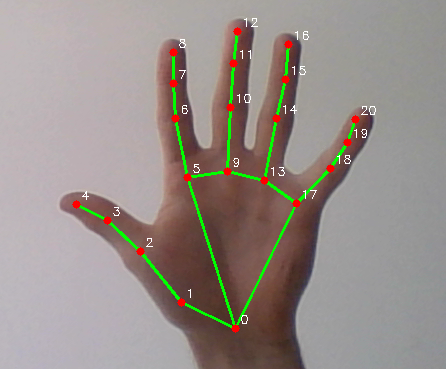
\includegraphics[width=0.9\textwidth]{material/figures/Mediapipe-HandPoints.png}
    \caption{Beispiel Hand Landmark Punkte | Eigene Darstellung}
    \label{fig:hand-landmarks}
\end{figure}

Zusätzlich gibt das Modell einen Handedness-Score aus, der angibt, ob es sich um eine linke oder rechte Hand handelt.

\subsection{Region of Interest}\label{sub:roi}

Eine ROI (Region of Interest) ist ein rotiertes Rechteck im Pixelraum, das genau definiert, welchen Bildausschnitt ein Modell fokussieren oder als Eingabe für ML Modelle dienen soll. Dies kann verwendet werden um Modelle gezielt auszuführen. \cite{OnDeviceRealTimeHand} 

\begin{figure}[H]
    \centering
    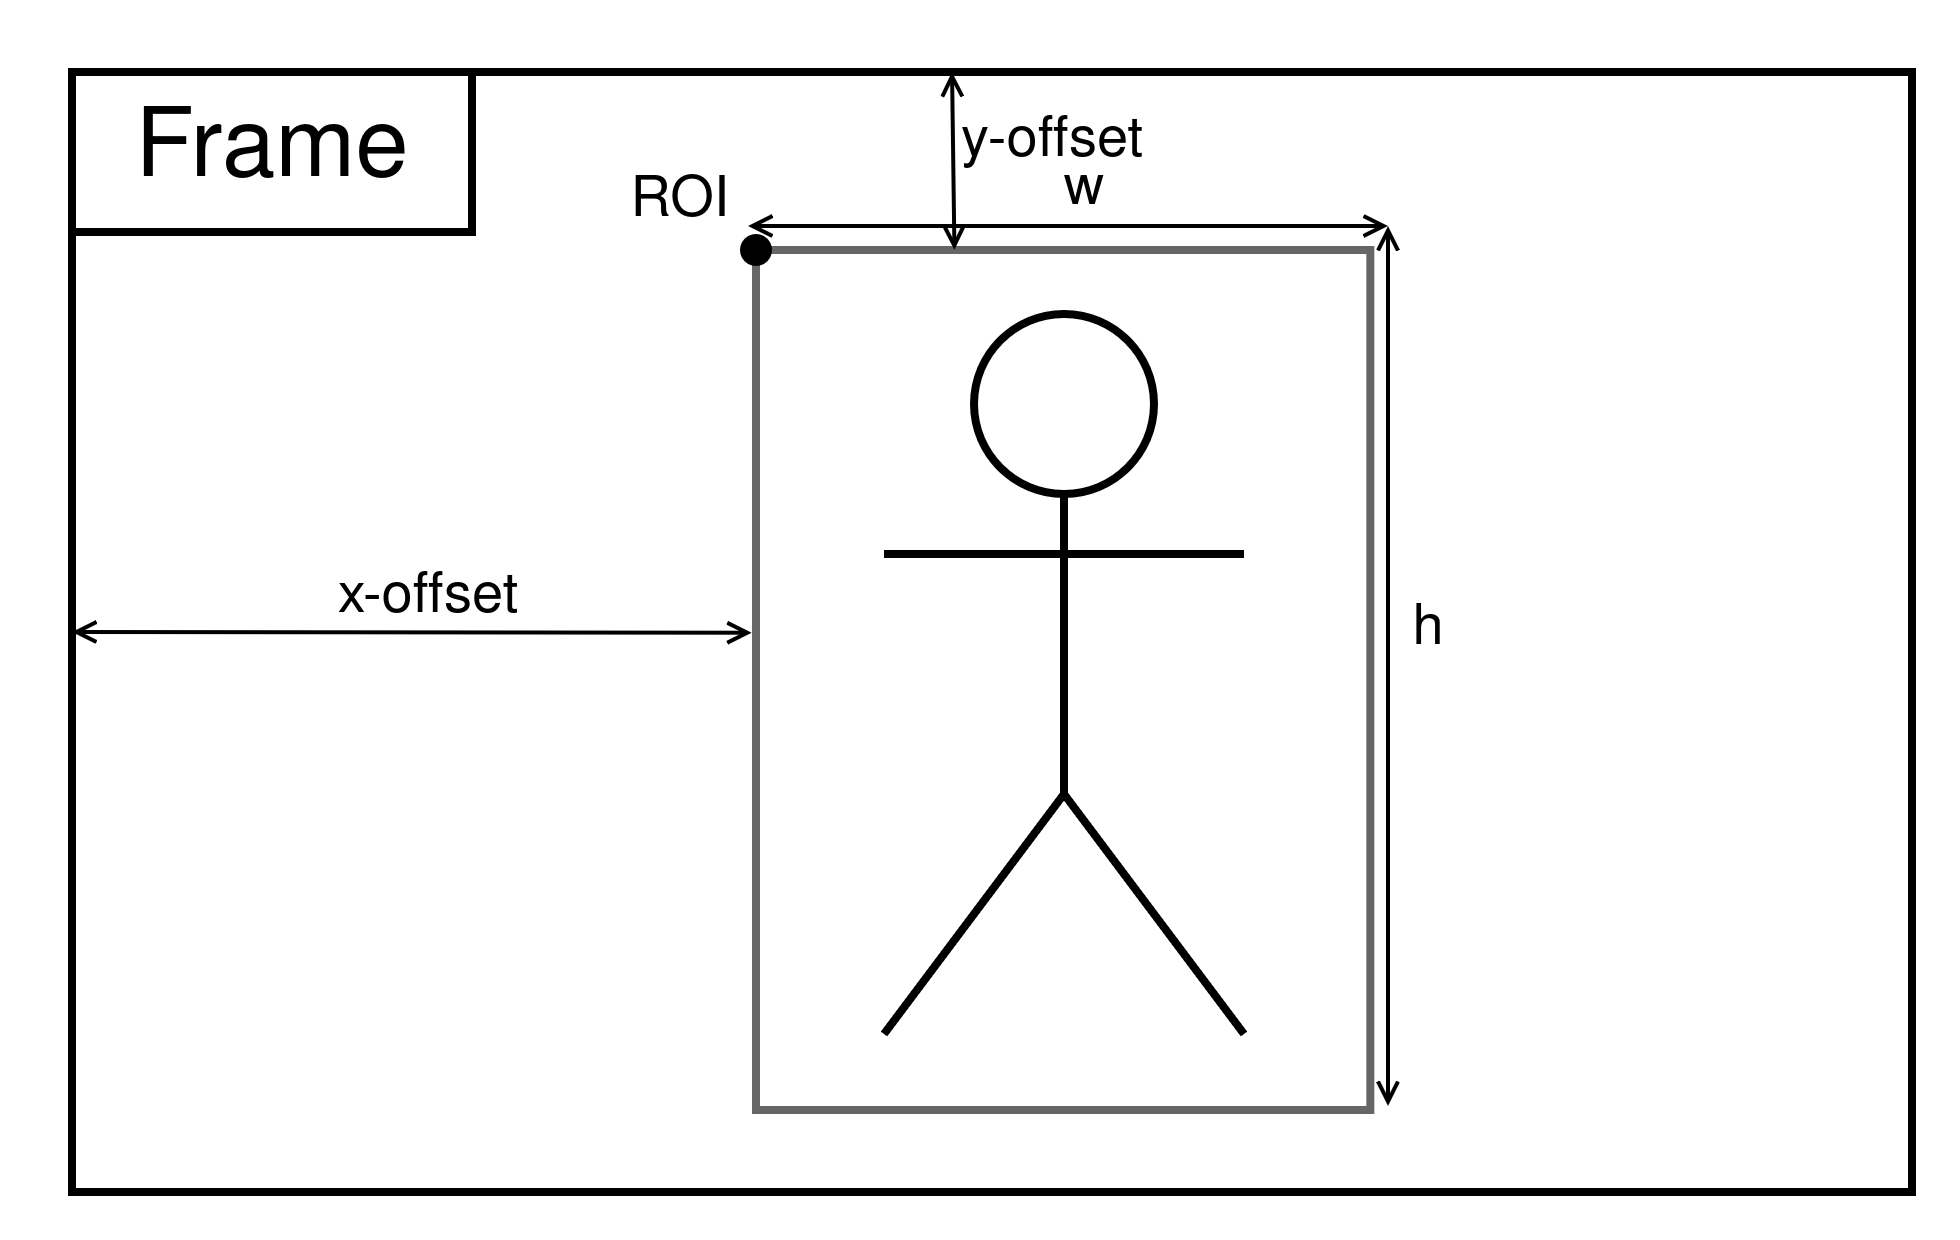
\includegraphics[width=0.9\textwidth]{material/figures/ROI-Explaination.png}
    \caption{ROI -- Example | Eigene Darstellung}
    \label{fig:roi-explaination}
\end{figure}

\subsubsection{Lifecycle}\label{ssub:roi-lifecycle}

Eine ROI entsteht durch die Ausgabe des Detector-Modells, das eine Bounding Box sowie Schlüsselpunkte liefert. Aus diesen werden Position, Orientierung und Größe der initialen ROI berechnet. In den folgenden Frames wird innerhalb der ROI das Landmark-Modell ausgeführt. Bei ausreichender Konfidenz des Landmark-Modells werden Landmarken in Bildkoordinaten zurückgerechnet und daraus eine aktualisierte ROI (Position, Orientierung, Größe) bestimmt. Dieser Vorgang wird jeden Frame wiederholt. Fällt die Konfidenz unter den definierten Schwellwert, wird die ROI verworfen und der Lifecycle endet.

\section{Datenaugmentation und Modellquantisierung}\label{sec:augmentation-quantisierung}

\subsection{Datenaugmentation}\label{sub:datenaugmentation}

\paragraph{Definition und Ziel:}
Datenaugmentation bezeichnet die künstliche Vermehrung eines Trainingsdatensatzes durch Transformationen der vorhandenen Daten. Der Zweck besteht darin, die Robustheit und Generalisierungsfähigkeit des Modells zu erhöhen, ohne zusätzliche Daten erfassen zu müssen. \cite{yingOverviewOverfittingIts2019}

\paragraph{Transformationsverfahren:} Im vorliegenden Projekt werden folgende Augmentationen eingesetzt:

\begin{itemize}
    \item Spiegelung (Horizontal Flip): Die Hand wird horizontal gespiegelt. Dies simuliert Unterschiede zwischen linker und rechter Hand sowie Variationen in der Handhaltung.
    \item Zufällige Translation: Die Landmarks werden um einen zufälligen Betrag in x- und y-Richtung verschoben, um unterschiedliche Handpositionen im Kamerabild zu simulieren.
    \item Zufälliger Zoom: Die Landmarks werden um einen Faktor zwischen 0,5$\times$ und 1,5$\times$ skaliert, um unterschiedliche Handgrößen und Abstände zur Kamera abzubilden.
    \item Jitter: Zufälliges Rauschen wird zu den Koordinaten hinzugefügt, um natürliche Schwankungen in der Landmark-Erkennung zu simulieren.
\end{itemize}

\paragraph{Implementierung:}
Die Augmentationspipeline (\texttt{AugmentationPipeline}) wendet diese Transformationen sequenziell auf die extrahierten Landmarks an und erzeugt pro Original-Datensatz mehrere Variationen. Dadurch wird der effektive Datensatz um einen Faktor von typisch 5--10$\times$ vermehrt.

\subsection{Modellquantisierung}\label{sub:modellquantisierung}

Neuronale Netze verwenden bei Training und Inferenz üblicherweise Fließkommazahlen um eine möglichst hohe Genauigkeit zu erreichen (Float32, 4 Byte pro Wert). Auf ressourcenbeschränkten eingebetteten Plattformen ist dies sowohl speichermäßig als auch rechnerisch ineffizient \cite{jacobQuantizationTrainingNeural2018}. Die Quantisierung reduziert die Genauigkeit der Gewichte und Aktivierungen auf Ganzzahlen (typisch INT8, 1 Byte pro Wert).

\begin{table}[H]
    \centering
    \label{tab:float32-vs-int8}
    \begin{tabular}{|p{0.35\textwidth}|l|l|}
        \hline
        \textbf{Eigenschaft} & \textbf{Float32} & \textbf{INT8} \\
        \hline
        Speicher pro Gewicht & 4 Byte & 1 Byte \\
        \hline
        Speicherersparnis & -- & 75\,\% \\
        \hline
        Rechengeschwindigkeit & Standard & Deutlich schneller (NPU-nativ) \\
        \hline
        Genauigkeit & Hoch & Leicht reduziert (hinnehmbar) \\
        \hline
    \end{tabular}
    \caption{Vergleich Float32 vs.\ INT8}
\end{table}

\begin{itemize}
    \item Scale und Zero-Point: Die Quantisierung bildet den Float32-Wertebereich auf einen Integer-Bereich ab
    \item Post-Training-Quantisierung (PTQ): Bei der Post-Training-Quantisierung wird ein bereits trainiertes Float32-Modell in ein INT8-Modell konvertiert, ohne erneutes Training \cite[Kap. 8-Quantization]{pointerPyTorchFuerDeep2020}. Dafür wird ein Repräsentativer Datensatz verwendet. Es handelt sich um eine Stichprobe der Trainingsdaten, anhand derer die Aktivierungsbereiche der Schichten analysiert und die optimalen Skalierungsfaktoren bestimmt werden.
    \item Genauigkeitsverluste: Die Reduktion von Float32 auf INT8 kann zu einem leichten Rückgang der Modellgenauigkeit führen. In der Praxis ist dieser Verlust bei geeigneter Kalibrierung (Repräsentativer Datensatz) jedoch gering (typisch < 2 \% Accuracy-Verlust) und für die meisten Anwendungsfälle akzeptabel.
\end{itemize}

\section{Edge AI und Neuronale Beschleuniger (NPU)}\label{sec:edge-ai}

\subsection{Edge AI}\label{sub:edge-ai-detail}

Edge AI bezeichnet die Ausführung von KI-Inferenzen direkt auf dem Endgerät \textit{(engl. edge device)} anstelle einer Übertragung der Daten an einen Cloud-Server \cite{smalleyWhatEdgeAI2023, abadadeComprehensiveSurveyTinyML2023}. Die Mikrocontroller erfassen Daten über Sensoren und verarbeiten diese lokal mithilfe von Modellen des maschinellen Lernens. Die wesentlichen Vorteile gegenüber Cloud-basierten Ansätzen sind:

\begin{itemize}
    \item Geringe Latenz: Die Verarbeitung erfolgt lokal, ohne Netzwerkübertragungszeit. Für Echtzeitanwendungen wie die Gesture-Erkennung ist dies essentiell.
    \item Datenschutz: Biometrische Daten (Kamerabilder der Hand) verlassen das Gerät nicht.
    \item Offline-Fähigkeit: Das System funktioniert ohne Internetverbindung.
    \item Reduzierte Bandbreite: Es müssen keine Bilder übertragen werden.
\end{itemize}

Die Haupt-Herausforderung liegt in der Ressourcenbeschränkung: Speicher, Rechenleistung und Energieverbrauch sind auf eingebetteten Plattformen stark limitiert. Ein KI-Modell, das auf einem Server mit Gigabytes an Speicher und leistungsstarken GPUs trainiert wurde, muss auf dem Mikrocontroller mit wenigen Kilobytes an SRAM und einem dedizierten Beschleuniger betrieben werden \cite{abadadeComprehensiveSurveyTinyML2023}.

\subsection{Neuronale Beschleuniger (NPU)}\label{sub:npu}

Der Neural-Art-Beschleuniger ist eine parametrierbare und zur Laufzeit rekonfigurierbare Neuronale Verarbeitunseinheit (NPU). Diese dedizierte Hardware-Einheit dient der Inferenz INT8 quantisierter Convolutional Neural Networks (CNN) \cite[S. 1011 ff.]{rm0486}. Im Gegensatz zur allgemeinen CPU, die nur einen Bruchteil ihrer Rechenleistung für Matrix-Operationen nutzt, führt die NPU Matrix-Multiplikationen, Vektoroperationen und spezialisierte CNN Instruktionen mit hoher Parallelität aus.

Die NPU arbeitet mit einer eigenen Speicherhierarchie: Die AXISRAM-Banken dienen als Puffer für Gewichte und Aktivierungen, sodass die NPU unabhängig von der CPU auf Daten zugreifen kann (vgl.\ Abschnitt~\ref{fig:stm32n6-architektur}).

Für die Ausführung der konvertierten Modelle stellt STMicroelectronics eine Laufzeitumgebung bereit, die als \textit{ATON-Runtime} bezeichnet wird. Sie lädt die generierten Netzwerk-Binaries, verwaltet deren Ein- und Ausgabepuffer und führt die einzelnen NPU-Epochen aus. Die Kommunikation zwischen Anwendungssoftware und den NPU-Komponenten erfolgt über eine Middleware \cite{STNeuralARTCompiler}

\subsection{ST Edge AI Core CLI}\label{sub:stedge-ai}

ST Edge AI Core ist ein Command Line Interface (CLI) das genutzt wird, um Convolutional Neural Networks (CNN) im ONNX (QDQ) oder TF-Lite-Format in ein für die NPU-Platform passendes Format zu überführen. Der ST Neural-ART-Compiler ist als Back-End in die ST Edge Core CLI integriert und führt alle Optimierungen, Graph-Planung und Code-Generierung offline durch. Es wird keine interpretierende Engine auf dem eingebetteten System ausgeführt.

\begin{figure}[H]
    \centering
    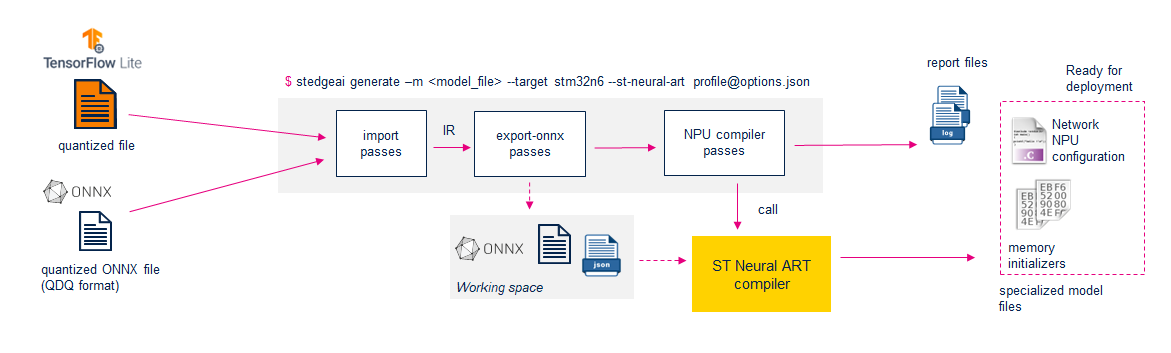
\includegraphics[width=0.9\textwidth]{material/figures/NPU-TF-Lite ONNX Model harware executable conversion.png}
    \caption{NPU -- Quantized Model Conversion to NPU Executables \cite{STNeuralARTCompiler}}
    \label{fig:npu-conversion}
\end{figure}

\begin{figure}[H]
    \centering
    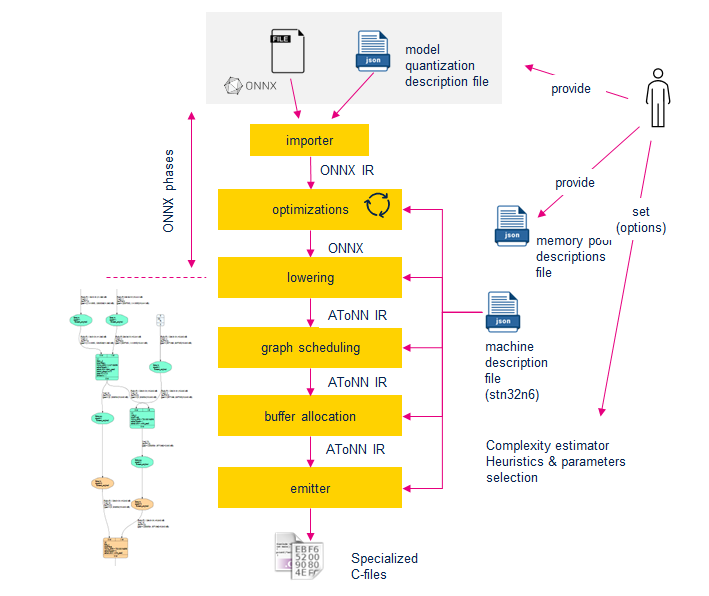
\includegraphics[width=0.9\textwidth]{material/figures/NPU-Compilation.png}
    \caption{NPU -- Compilation \cite{STNeuralARTCompiler}}
    \label{fig:npu-compilation}
\end{figure}

Modelle werden in NPU-Epochen unterteilt die in die verfügbaren Hardwareressourcen abbilden. Die Umsetzung der Transformation geschieht mittels Mapping von TF-Lite/ONNX-Befehlen auf Epochen. Folgende Epochen werden unterschieden:

\begin{table}[H]
    \centering
    \label{tab:npu-epochen}
    \begin{tabular}{|p{0.2\textwidth}|p{0.7\textwidth}|}
        \hline
        \textbf{Epochen-Typ} & \textbf{Beschreibung} \\
        \hline
        HW-Epochen & Operatoren vollständig auf NPU-Hardware abgebildet. Die MCU-Arbeitslast beträgt ca.\ 10--15\,\% der Inferenzzeit. \\
        \hline
        SW-Epochen & Operatoren an Host delegiert (Keine Beschleunigung). \\
        \hline
        Hybrid-Epochen & Teilweise Software, teilweise hardwareunterstützt über vordefinierte Hardware-Epochen. \\
        \hline
        Meta-Epochen & Menge von Hardware-Epochen, gesteuert über Befehlsstrom via Epochen-Controller. \\
        \hline
    \end{tabular}
    \caption{NPU-Epochen-Typen}
\end{table}

Epochen werden als atomare Operationen in fester Reihenfolge ausgeführt, um Datenabhängigkeiten zu gewährleisten. Zwischen Epochen wird kein interner NPU-Hardware-Zustand erhalten. Zwischenergebnisse werden im externen Speicher abgelegt.
